\section{Orders}

Die Orderseite erlaubt es, getätigte Bestellungen von Nutzern pro Tag einzusehen.

\begin{figure}[ht]
    \centering
    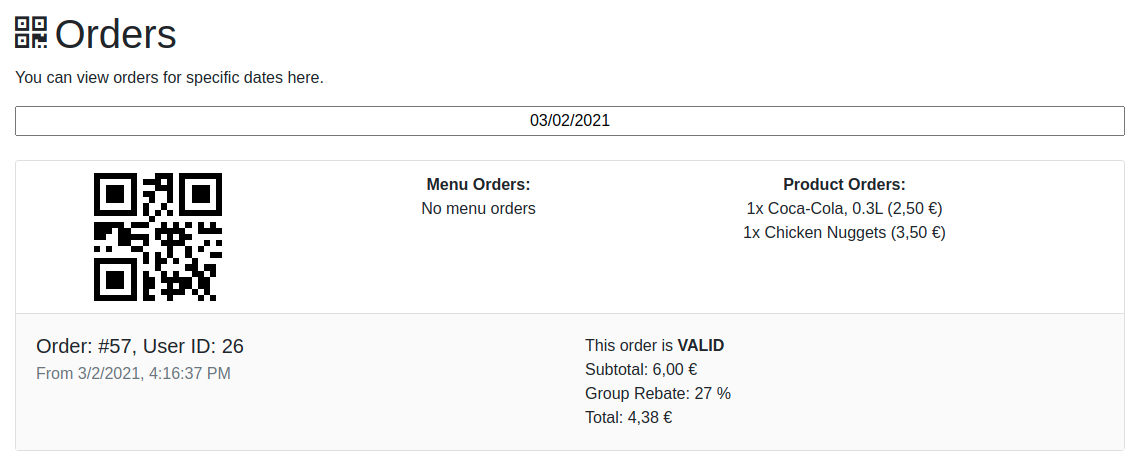
\includegraphics[width=0.8\textwidth]{images/ACP/orders.png}
    \caption{Die Bestellungsseite des Sokka-ACPs}
\end{figure}

Die Order-Seite des ACPs ist rein informativ. Hier können keine Änderungen an den Bestellungen vorgenommen werden, beispielsweise können Bestellungen im ACP nicht invalidiert werden. Für das Bearbeiten von Bestellungen existiert der \textit{\nameref{adminclient}}.

Das ACP zeigt folgende Informationen pro Bestellung an:

\begin{itemize}
    \item Die ID der Bestellung
    \item Die ID des Nutzers, der die Bestellung getätigt hat
    \item Den Zeitpunkt der Bestellung
    \item Den Inhalt der Bestellung
    \item Den Preis und Rabatt der Bestellung
    \item Die Validität der Bestellung (\textbf{VALID} bedeutet, dass die Bestellung noch nicht eingelöst wurde, \textbf{INVALIDATED} bedeutet, dass die Bestellung an der Kasse eingelöst wurde)
\end{itemize}

Der QR-Code ergibt sich aus der Bestellungs-ID und der Nutzer-ID im Format \lstinline{<userID>:<orderID>} und ist derselbe QR-Code, der auch im Client angezeigt wird.

\begin{figure}[ht]
    \centering
    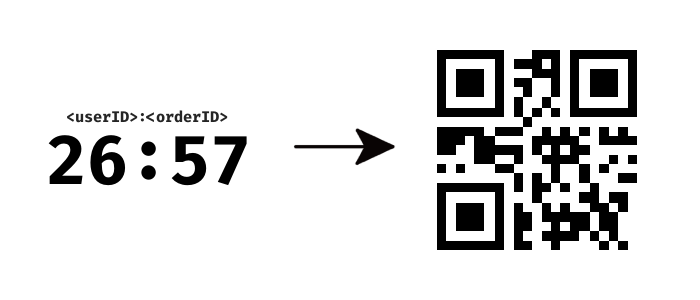
\includegraphics[width=0.7\textwidth]{images/ACP/arrow.png}
    \caption{QR-Code-Erstellung der Bestellungen}
\end{figure}